\def\year{2021}\relax
%File: formatting-instructions-latex-2021.tex
%release 2021.2
\documentclass[letterpaper]{article} % DO NOT CHANGE THIS
\usepackage{aaai21}  % DO NOT CHANGE THIS
\usepackage{times}  % DO NOT CHANGE THIS
\usepackage{helvet}
\usepackage{graphicx} % for '\resizebox` macro
\usepackage{array}
\usepackage{hyperref}
\hypersetup{
    colorlinks=true,
    linkcolor=black,
    filecolor=magenta,      
    urlcolor=gray,
    pdftitle={Overleaf Example},
    pdfpagemode=FullScreen,
    }

\usepackage[table]{xcolor}% DO NOT CHANGE THIS
\usepackage{courier}  % DO NOT CHANGE THIS
\usepackage[hyphens]{url}  % DO NOT CHANGE THIS
\urlstyle{rm} % DO NOT CHANGE THIS
\def\UrlFont{\rm}  % DO NOT CHANGE THIS
\usepackage{natbib}  % DO NOT CHANGE THIS AND DO NOT ADD ANY OPTIONS TO IT
\usepackage{caption} % DO NOT CHANGE THIS AND DO NOT ADD ANY OPTIONS TO IT
\usepackage{amssymb}
\frenchspacing  % DO NOT CHANGE THIS
\setlength{\pdfpagewidth}{8.5in}  % DO NOT CHANGE THIS
\setlength{\pdfpageheight}{11in}  % DO NOT CHANGE THIS
\usepackage{float}
%\nocopyright
%PDF Info Is REQUIRED.
% For /Author, add all authors within the parentheses, separated by commas. No accents or commands.
% For /Title, add Title in Mixed Case. No accents or commands. Retain the parentheses.
\pdfinfo{
/Title (AAAI Press Formatting Instructions for Authors Using LaTeX -- A Guide)
/Author (AAAI Press Staff, Pater Patel Schneider, Sunil Issar, J. Scott Penberthy, George Ferguson, Hans Guesgen, Francisco Cruz, Marc Pujol-Gonzalez)
/TemplateVersion (2021.2)
} %Leave this
% /Title ()
% Put your actual complete title (no codes, scripts, shortcuts, or LaTeX commands) within the parentheses in mixed case
% Leave the space between \Title and the beginning parenthesis alone
% /Author ()
% Put your actual complete list of authors (no codes, scripts, shortcuts, or LaTeX commands) within the parentheses in mixed case.
% Each author should be only by a comma. If the name contains accents, remove them. If there are any LaTeX commands,
% remove them.

% DISALLOWED PACKAGES
% \usepackage{authblk} -- This package is specifically forbidden
% \usepackage{balance} -- This package is specifically forbidden
% \usepackage{color (if used in text)
% \usepackage{CJK} -- This package is specifically forbidden
% \usepackage{float} -- This package is specifically forbidden
% \usepackage{flushend} -- This package is specifically forbidden
% \usepackage{fontenc} -- This package is specifically forbidden
% \usepackage{fullpage} -- This package is specifically forbidden
% \usepackage{geometry} -- This package is specifically forbidden
% \usepackage{grffile} -- This package is specifically forbidden
% \usepackage{hyperref} -- This package is specifically forbidden
% \usepackage{navigator} -- This package is specifically forbidden
% (or any other package that embeds links such as navigator or hyperref)
% \indentfirst} -- This package is specifically forbidden
% \layout} -- This package is specifically forbidden
% \multicol} -- This package is specifically forbidden
% \nameref} -- This package is specifically forbidden
% \usepackage{savetrees} -- This package is specifically forbidden
% \usepackage{setspace} -- This package is specifically forbidden
% \usepackage{stfloats} -- This package is specifically forbidden
% \usepackage{tabu} -- This package is specifically forbidden
% \usepackage{titlesec} -- This package is specifically forbidden
% \usepackage{tocbibind} -- This package is specifically forbidden
% \usepackage{ulem} -- This package is specifically forbidden
% \usepackage{wrapfig} -- This package is specifically forbidden
% DISALLOWED COMMANDS
% \nocopyright -- Your paper will not be published if you use this command
% \addtolength -- This command may not be used
% \balance -- This command may not be used
% \baselinestretch -- Your paper will not be published if you use this command
% \clearpage -- No page breaks of any kind may be used for the final version of your paper
% \columnsep -- This command may not be used
% \newpage -- No page breaks of any kind may be used for the final version of your paper
% \pagebreak -- No page breaks of any kind may be used for the final version of your paperr
% \pagestyle -- This command may not be used
% \tiny -- This is not an acceptable font size.
% \vspace{- -- No negative value may be used in proximity of a caption, figure, table, section, subsection, subsubsection, or reference
% \vskip{- -- No negative value may be used to alter spacing above or below a caption, figure, table, section, subsection, subsubsection, or reference

\setcounter{secnumdepth}{0} %May be changed to 1 or 2 if section numbers are desired.

% The file aaai21.sty is the style file for AAAI Press
% proceedings, working notes, and technical reports.
%

% Title

% Your title must be in mixed case, not sentence case.
% That means all verbs (including short verbs like be, is, using,and go),
% nouns, adverbs, adjectives should be capitalized, including both words in hyphenated terms, while
% articles, conjunctions, and prepositions are lower case unless they
% directly follow a colon or long dash


\title{Genetic Algorithm to understand evolution on the mutation of the proteins}
\author {
    % Author
    Piermarco Giustini 
}

\begin{document}

\maketitle

\begin{abstract}

\noindent Precise mRNA splicing is required for proper protein translation. Point mutations in sequences can result in incorrect recognition and the creation of an abnormal transcript of the altered gene. Typically, such mutations induce mistakes during the splicing process, which might affect the open reading frame. So the Genetic algorithm nearly perfectly describes this type of problem: we have a set population of proteins and we want to understand where the mutations come from. As a result, the major purpose is to rebuild the likely step that led to the mutation from a mutated and provided population using the logic of a Genetic Algorithm.

\end{abstract}

\section{Project Purpose}
Some $DNA$ $mutations$ are quiet and have no impact, but others influence protein, which regulates whether the gene is active or not, produces more or less protein or changes protein synthesis entirely. A mutation is a change in a DNA sequence caused by either a mistake during DNA replication or chemical damage. Genes are regions of the genome that contain instructions for the synthesis of protein molecules, which perform the majority of the vital functions in cells. Understanding the cause of a mutation of a certain section of DNA can lead to understanding what happened during the history of protein mutation.
By constructing a $big$ $pool$ $of$ $string$ $of$ $Genes$, this algorithm will be able to quickly identify what is likely the protein where the mutation came from.

\section{How it is done}
Genetic Algorithms are adaptive heuristic search algorithms that are a subset of $evolutionary algorithms$. These are clever exploitations of random search given with historical data to lead the search into the solution space area of greater performance. 
In other words, they replicate "survival of the fittest" among individuals of successive generations in order to solve a problem. 
Each generation is made up of a population of individuals, with each individual representing a point in the search space and a potential solution. Every person is represented by a string of character/integer/float/bits. This string is similar to the Chromosome. 
\section{Creation of The Population}
For this part, it is really important to define a $optimal solution$ and a $population$ that correspond to a list of $chromosome$ of the same length of the optimal solution:
\[population = {'AGTT', 'AGTT', ...}\]
\[chromosome = {'AGTT'}\]
\[optimal = {'ACCC'}\]
\section{Fitness Function}
Each new generation has more $superior genes$ on average than the individual (solution) of prior generations. As a result, each successive generation has better $partial answers$ than prior generations. This is translated in our instance because we are mutating in the right way to discover a perfect matching chromosome with the optimal solution. The underlying difficulty with this fitness score function is that there is no standard method to write it.
Looking online, many people claim that writing a fitness function is really difficult, however there is one that works the majority of the time, by using the absolute value between each chromosome and the optimal solution.\\
\begin{table}[h]
    \centering
    \begin{tabular}{c|c}
         A & 65 \\
         G & 71\\
         T & 84 \\
         C & 67 \\
         U & 85
    \end{tabular}
    \caption{ASCII code for nucleotides}
    \label{tab:my_label}
\end{table}
\[ absolute = |A - G| = |65 - 71| = 6 \]
\section{Evolution}
Once the fitness function is defined, the next step is to conduct two critical operations that allow the algorithm to develop without assistance. The first operation that was developed was the $crossover$, which consisted of flipping a portion of two chromosomes by putting two cross sites. This process is carried out on the chromosome with the highest $fitness score$ using a random choice probability, such that the next population generated is closer to the solution.\\
\[{'\textbf{AGTTCT}'}, {'ACCCTG'}\]
\[crossover index = {1:3}\]
\[{'\textbf{A}CCC\textbf{CT}'},{'A\textbf{GTT}TG'}\] \\
The other operation is termed $mutation$, and it was one of the most critical parameters to fix during the experiment since a high mutation rate resulted in the failure to discover a solution. Using a low mutation rate, on the other hand, results in merely a permutation owing to the crossover operation and the method get stack.\\ 
\['AGTCCTC ---> \textbf{C}GTCCT\textbf{A} \] \\
\section{Algorithm}
\begin{enumerate}
    \item Define the optimal protein
    \item Create the population
    \item Define fitness score function 
    \item Until don't find optimal protein:
    \begin{enumerate}
        \item Select 2 most chromosome based on their fitness score try to catch the best ones
        \item Perform crossover operation and mutation operation
        \item place the 2 new chromosome in the population
        \item calculate the fitness for the population 
    \end{enumerate}
\end{enumerate}


\section{I tools used in the project}
What is used during the experiment:
\begin{itemize}
\item VScode
\item \href{https://github.com/Reevoc/ARTIFICIAL-INTELLIGENCE/blob/main/Genetic%20Algorithm.ipynb}{GitHub}
\item Python 
\item Jupiter Notebook
\end{itemize}

\section{Experiments}
It is possible to see how the experiment is carried out by looking at the table in the following pages. The experiments are carried out by choosing an optimal protein to locate and test with a different kind of parameter. Two different types of graphs are displayed. The first demonstrates the development of the learning trend and how we are approaching the answer age after era. The other, in contrast, demonstrates the variation between the most recent population of all proteins generated and the ideal one. The difference from the ideal one increases with the height of the histogram bar.

\section{Future work}
A well-known protein could be used in the work's future iterations in order to see if the final population produced by the genetic algorithm has any well-known "mutated" proteins from the original.

\begin{figure}[h]
\centering
    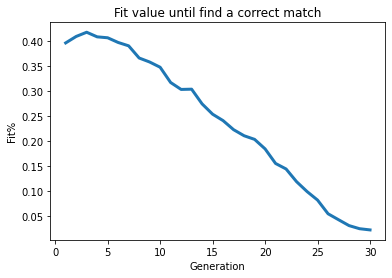
\includegraphics[scale = 0.5]{fitpop100.png}
    \caption{experimet 1}
\end{figure}
\begin{figure}[h]
 \centering
 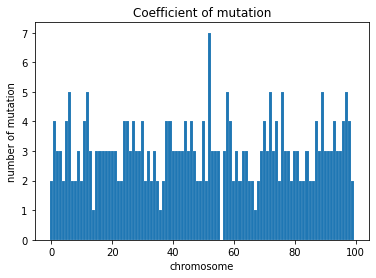
\includegraphics[scale = 0.5]{histpop100.png}
    \caption{experimet 1}
\end{figure}
\begin{figure}[h]
\centering
    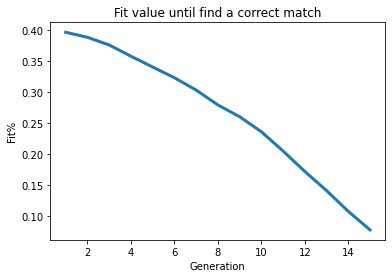
\includegraphics[scale = 0.5]{fitpop1000.png}
    \caption{experimet 2}
\end{figure}
\begin{figure}[h]
 \centering
 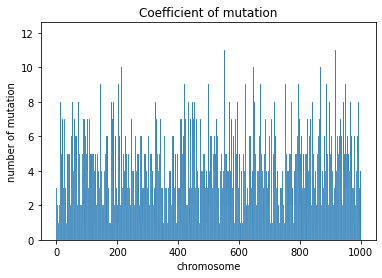
\includegraphics[scale = 0.5]{histpop1000.png}
 \caption{experimet 2}
\end{figure}
\begin{figure}[h]
\centering
    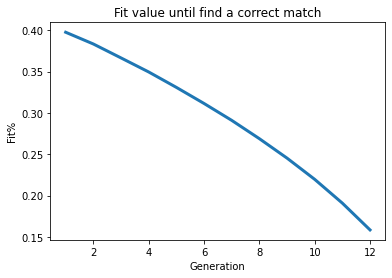
\includegraphics[scale = 0.5]{fitpop 10000.png}
    \caption{experimet 3}
\end{figure}
\begin{figure}[h]
 \centering
 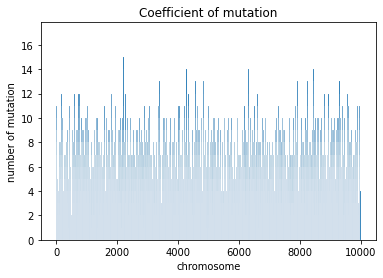
\includegraphics[scale = 0.5]{histpop 10000.png}
 \caption{experimet 3}
\end{figure}
\begin{figure}[h]
\centering
    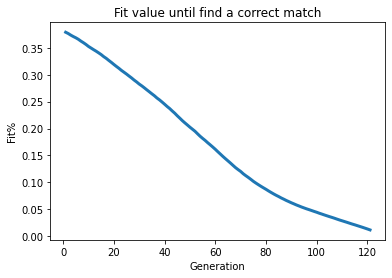
\includegraphics[scale = 0.5]{fitpop10000v2.png}
    \caption{experimet 4}
\end{figure}
\begin{figure}[h]
 \centering
 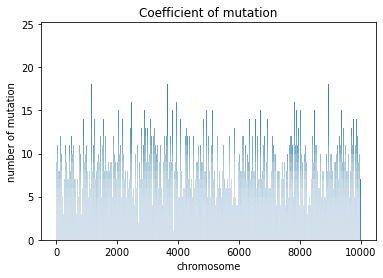
\includegraphics[scale = 0.5]{histpop10000v2.png}
 \caption{experimet 4}
\end{figure}

\begin{table*}[t]
\centering
\begin{tabular}{|c|c|c|c|c|c|}
        \hline
            Experiment & length opt & Correct Epoch & Num population & Max dif genes & time \\
            \hline
            exp1& 20 & 30 & 100 & 0.35 & 0.3s \\
            exp2& 20 & 15 & 1000 & 0.6 & 1.7s \\
            exp3& 20 & 12 & 10000 & 0.75 & 3m42.3s\\
            exp4& 100 & 121 & 10000 & 0.24 & 38m 13.2s\\
            \hline
    \end{tabular}
    \caption{Four tests were carried out utilizing the genetic algorithm, where length opt is the overall length of the optimum Protein that we wish to find. Correct Epoch is the precise epoch at which the correct answer is discovered (also in the code the population is saved), The population number is the first population formed (e.g. 100 random strings created at the beginning), Max dif genes is the maximum difference between the genes that differ (e.g., $0.35$ signifies that the gene varies by $35\%$ from the right one), and time is the time required to assess the proper answer.}
\end{table*}

\section{References}
\begin{quote}
\begin{small}
\textbackslash bibliography\{mybib.bib\}
\end{small}
\end{quote}




\end{document}
 